\documentclass{article}
\usepackage{url}
\usepackage{tikz}
\usetikzlibrary{arrows,positioning}

\begin{document}
\title{OpenTimestamps}
\author{Peter Todd}
\date{June 24 2012}
\maketitle

\begin{abstract}
Prior timestamping schemes have either assumed a single, trusted entity, or a
distributed set of trusted entities, that in turn trust each other. Here we
introduce a distributed timestamping scheme allowing multiple, entities, who
may or may not trust each other, and may or may not have reliable connectivity,
to collaborate to create timestamps whose falsification would require the
participation of every entity in the scheme.
\end{abstract}

\section{Background}

\subsection{PKI-based timestamps}

Digital timestamping allows one to prove that some data $D$ existed before some
time $T$. Haber and Stornetta proposed\cite{Haber91howto} the first usable
scheme depending on the existence of cryptographic hash functions. Such a
function $H$ has can be applied to an arbitrarily large string, producing a
digest: $d=H(D)$ with the property that computing $H(D)$ is easy, finding
another $D'$ such that $H(D)=H(D')$ is infeasible. \footnote{In fact, finding
any two strings $x$ and $x'$ such that $H(x)=H(x')$ is infeasible.} Haber
proposes that once the digest has been computed it can be sent to a remote
server who then replies with a signature $s=S(d\| t)$ of both the digest, and a
time. Anyone else can now easily verify the signature and, assuming they trust
the entity that created it, verify that the data existed before that time. An
example of these scheme in actual practice is seen in RFC3161.\cite{rfc3161}
Note that we have not specified exactly what form the signature takes, except
that there is some function $V$ which given $s$ and $d\| t$ can verify the
latter.

While this scheme has the advantage of simplicity and small timestamps there
are some serious disadvantages as well. First of all the scalibility is poor,
as any given timestamping server can only serve a limited number of requests
per second; increasing this limit requires more servers and hence more
opportunity for key compromise. Secondly the server is absolutely trusted, and
can create forged timestamps after the fact.

A final disadvantage is caused by possible compromise of the hash function. For
instance someone implementing a Haber's scheme in 1991, using cryptography
known to the public, could have chosen MD4 as the hash function. Unfortunately
MD4 was broken in 2004 and generating an $x,x'$ such that
$H_{MD4}(x)=H_{MD4}(x')$ is now possible in a few
microseconds.\cite{Wang05cryptanalysisof} In addition a preimage attack, where
a $D'$ is found from an arbitrary $D$ such that $H_{MD4}(D)=H_{MD4}(D')$ has
also been found with $2^{102}$ complexity.\cite{Leurent_md4is} While this in
itself does not invalidate \emph{existing} timestamps, as finding $D'$ to
colide with an existing $D$ is still very difficult, and the timestamp itself
shows that $H_{MD4}(D)$ was created before such an attack was known, it does
suggest that future advancements in cryptanalysis will make those timestamps
untrustworthy.

\subsection{Linear-linking schemes}

\begin{figure}
    \centering
    \usetikzlibrary{arrows,positioning}
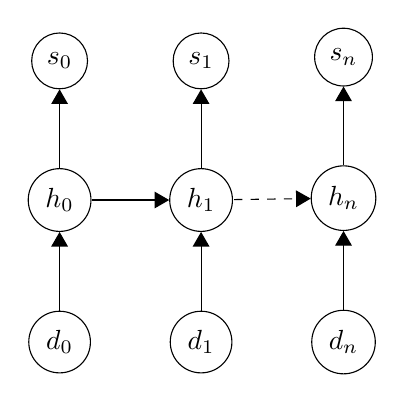
\begin{tikzpicture}[every node/.style={circle,draw},
                                    every path/.style={<-,>=triangle 60}]

\node (d0) {$d_0$};
\node[right=of d0] (d1) {$d_1$};
\node[right=of d1] (dn) {$d_n$};

\node[above=of d0] (h0) {$h_0$} edge (d0);
\node[above=of d1] (h1) {$h_1$} edge (d1) edge (h0);
\node[above=of dn] (hn) {$h_n$} edge (dn) edge[dashed] (h1);

\node[above=of h0] (s0) {$s_0$} edge (h0);
\node[above=of h1] (s1) {$s_1$} edge (h1);
\node[above=of hn] (sn) {$s_n$} edge (hn);

\end{tikzpicture}
    \caption{A simple linear linking scheme}
    \label{fig:linear-linking-scheme}
\end{figure}

To detect forgery by the server Haber proposed an extension, shown in figure
\ref{fig:linear-linking-scheme}, known as a linear linking
scheme.\cite{Haber91howto} Here $h_i=H(h_{i-1} \| d_i)$ with signature
$s_i=S(h_i)$. If the timestamp server periodically publishes the full list of
hashes and signatures, (the "calendar") a later forgery of a signature $s_k$
can be detected by noting that $h_{k-1}$ and $h_{k+1}$ are not in the
previously published calendar. However the calendar will be quite large,
scaling linearly with the total number of timestamps ever issued.

\subsection{Binary-linking schemes}

To overcome the large size of the calendar in a linear linking scheme, as well
as the inherent performence problems of a single timestamping server, a scheme
based on binary schemes has been proposed.\cite{Buldas98time-stampingwith} As
before we have a linearly linked calendar, $c_i$, however instead of including
digests directly in the calendar we construct a tree of digests, with each
vertex of the tree being the hash of the concatenation of the digests under
it.\footnote{This structure is also more generally known as a merkle tree.\cite{merkle87}} A
timestamp now comprises the signature $s_i$ as well as the digests of the
vertices (shown in bold) that lead to the calendar entry $c_i$.  Verification
consists of recreating $c_i$ by hashing the saved vertices, then verifying
that $s_i$ is a valid signature of $c_i$ and the time.

Provided the tree is balanced, the number of vertices in a timestamp will scale
by $\log_2 (n)$ with $n$ being the number of timestamps issued in the time
period between top level calendar entries. For an example of how scalable this
is, consider a timestamping server with a calendar interval of 1 second,
issuing $65,000 \approx 2^{16}$ timestamps per second, using SHA256 hashes:

\begin{equation}
(\log_2(2^{16})+1) \mathrm{Hashes} * \frac{256 \mathrm{Bits}}{\mathrm{Hash}} = 544
\mathrm{Bytes}
\end{equation}

This is not significantly more than an RSA signature. In addition unlike the
linear scheme the tree can be created by multiple timestamping servers working
in parallel, with only the server maintaining the actual calendar having to
hold the signing key. The disadvantage is that the resolution of the timestamp
is limited to the calendar interval.

\begin{figure}
    \centering
    \usetikzlibrary{arrows,positioning}
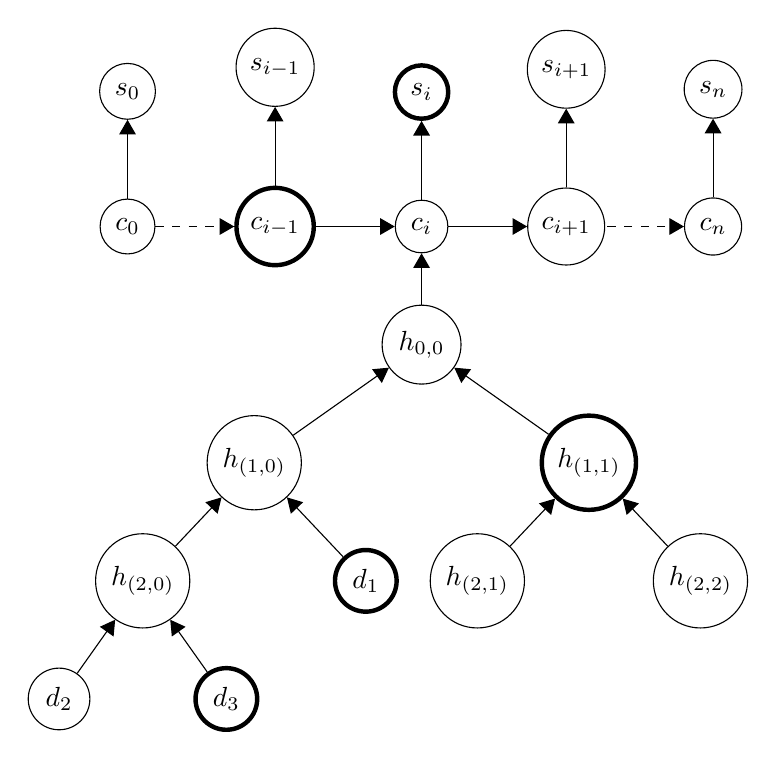
\begin{tikzpicture}[level/.style={sibling distance=85mm/#1}, 
                                    every node/.style={circle,draw},
                                    every path/.style={<-,>=triangle 60}]
\node (ci) {$c_i$}
child {node (h00){$h_{0,0}$}
  child {node (h10) {$h_{(1,0)}$}
    child {node (h20) {$h_{(2,0)}$}
      child {node (d2) {$d_2$}}
      child {node [ultra thick] (d3) {$d_3$}}
    }
    child {node [ultra thick] (h20) {$d_1$}}
  }
  child {node [ultra thick] (h11) {$h_{(1,1)}$}
    child {node (h21) {$h_{(2,1)}$}}
    child {node (h22) {$h_{(2,2)}$}}
  }
};

\node[above=of ci,ultra thick] (sn) {$s_i$} edge(ci);

\node[left=of ci,ultra thick] (ciminus) {$c_{i-1}$} edge[->] (ci);
\node[right=of ci] (ciplus) {$c_{i+1}$} edge[<-] (ci);

\node[above=of ciminus] (siminus) {$s_{i-1}$} edge (ciminus);
\node[above=of ciplus] (siplus) {$s_{i+1}$} edge (ciplus);

\node[left=of ciminus] (c0) {$c_0$} edge[->,dashed] (ciminus);
\node[right=of ciplus] (cn) {$c_n$} edge[<-,dashed] (ciplus);

\node[above=of c0] (s0) {$s_0$} edge (c0);
\node[above=of cn] (sn) {$s_n$} edge (cn);

\end{tikzpicture}
    \caption{A binary linking scheme, with a linearly linked calendar}
    \label{fig:three-level-merkle}
\end{figure}


\subsection{Signatures}

So far we have not discussed what exactly are signatures. While cryptographic
signatures, using public key cryptography, are an obvious solution, others
exist as well. For instance consider the signature function
$S_{\mathrm{Financial Times}}(d,t)$ which when given a digest and a time
returns the string "Published in the Financial Times, (some date)" within a few
weeks. The verification function $V_{\mathrm{Financial Times}}$ now consists of
asking some intern to run off to the local libraries archives, and an attack on
the integrity of the timestamp now requires a co-ordinated physical operation.
One example of such a scheme is shown in Figure \ref{fig:guardtime_20120615}.

\begin{figure}
    \centering
    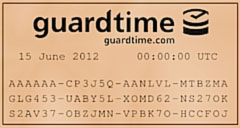
\includegraphics{figures/guardtime_20120615.jpg}
    \caption{A Guardtime publication code, allegedly published June 15 2012 in
    the World Edition of the Financial Times.}
    \label{fig:guardtime_20120615}
\end{figure}

In Guardtime's implementation, the 1 second interval calendar is fed into a 1
month interval calendar, using a "meta" binary tree. A user who submits a
digest for timestamping receives back a digest included in the 1 second
interval calendar, signed by a Guardtime server. At a later date the user can
"extend" this timestamp by requesting the vertices of the hash tree between the
1 second calendar entry, and the 1 month calendar entry published in the
Financial Times.  Verification can now operate at two levels, verification that
the timestamp was created within the 1 second claimed, and a more in-depth (and
manual) verification that the total hash chain leads to the 1 month
publication.\cite{guardtime-tech-overview}

\subsubsection{Proof-of-work signatures}

\begin{figure}
        \centering
        \usetikzlibrary{arrows,positioning}
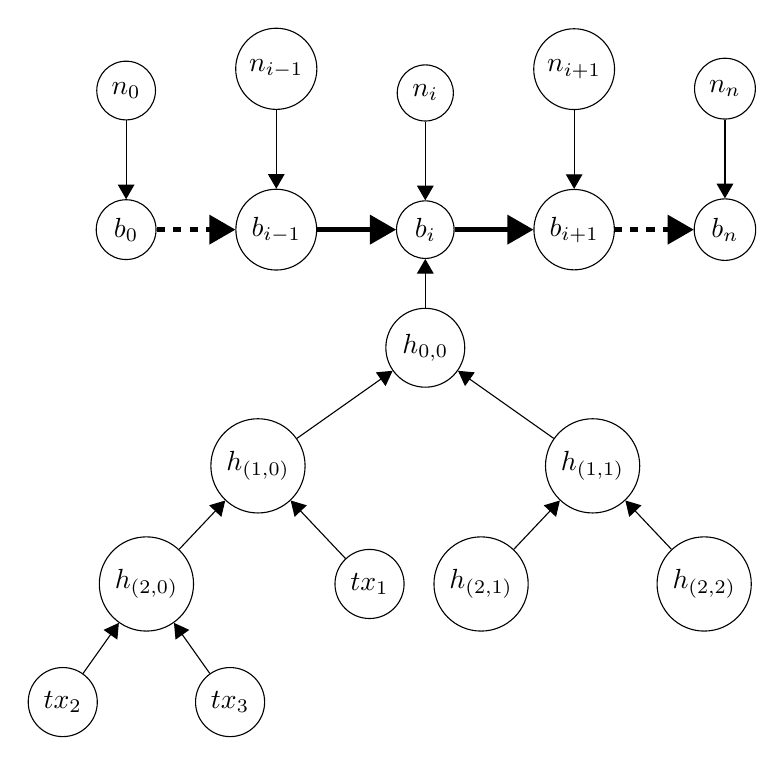
\begin{tikzpicture}[level/.style={sibling distance=85mm/#1}, 
                                    every node/.style={circle,draw},
                                    every path/.style={<-,>=triangle 60}]
\node (bi) {$b_i$}
child {node (h00){$h_{0,0}$}
  child {node (h10) {$h_{(1,0)}$}
    child {node (h20) {$h_{(2,0)}$}
      child {node (t2) {$tx_2$}}
      child {node (t3) {$tx_3$}}
    }
    child {node (h20) {$tx_1$}}
  }
  child {node (h11) {$h_{(1,1)}$}
    child {node (h21) {$h_{(2,1)}$}}
    child {node (h22) {$h_{(2,2)}$}}
  }
};

\node[left=of bi] (biminus) {$b_{i-1}$} edge[->,ultra thick] (bi);
\node[right=of bi] (biplus) {$b_{i+1}$} edge[<-,ultra thick] (bi);

\node[left=of biminus] (b0) {$b_0$} edge[->,dashed,ultra thick] (biminus);
\node[right=of biplus] (bn) {$b_n$} edge[<-,dashed,ultra thick] (biplus);

\node[above=of b0] (n0){$n_0$}edge[->] (b0);
\node[above=of biminus] (n0){$n_{i-1}$}edge[->] (biminus);
\node[above=of bi] (n0){$n_{i}$}edge[->] (bi);
\node[above=of biplus] (n0){$n_{i+1}$}edge[->] (biplus);
\node[above=of bn] (n0){$n_{n}$}edge[->] (bn);

\end{tikzpicture}
        \caption{The Bitcoin blockchain}
        \label{fig:bitcoin-overview}
\end{figure}

There is one unique category of "published" signatures that don't require
interns to find copies of physical artifacts for verification: Bitcoin.
Specifically what makes Bitcoin unique is that it provides a way to uniquely
order financial transactions such that the order of transactions is
unchangable. It does this in such a way that even completely untrusted
participants can work together to achieve consensus.\cite{Nakamoto_bitcoin:a}
Figure \ref{fig:bitcoin-overview} shows the basic structure what is known as
the Bitcoin blockchain; quite similar to the binary linking scheme shown in
figure \ref{fig:three-level-merkle}. Transactions, shown as $tx_i$, are
messages signed by keys stating that funds should be transfered from one
account to another. These transactions are combined with a merkle tree. At the
top level are the blocks in the blockchain, where each block digest
$b_i=H(h_{0,0} \| b_{i-1} \| n_i \| t)$. The security comes from nonce $n_i$,
which is chosen such that the first $k$ bits of $b_i$ are equal to $0$; the
proof-of-work. The Bitcoin network automatically adjusts $k$ such that even
with the combined efforts of tens of thousands of specialized
"miners",\footnote{As of June 2012 the latest in mining hardware uses FPGAs,
and multiple efforts to build custom ASICs are underway.} trying to compute
hashes, only about one block ever 10 minutes is generated. As part of algorithm
that adjusts $k$, each block also has a timestamp $t$, and participants in the
network will refuse to accept blocks whose timestamp is more than two hours
different from their local idea of time. In practice this means that each block
has a reasonably accurate timestamp.

The ultimate goal here is so that an attempt to spend money, which involves the
creation of a signed message stating that money can be moved from one account
to another, can be verified by waiting until that transaction has been "buried"
multiple blocks deep. Once this is true, the recepient can be assured that the
sender won't try to defraud them by sending the funds to another person, known
as a double spend attack. Of course, with around a million US dollars worth of
funds being transfered every day (as of June 2012), this represents tremendous
trust that this proof-of-work system works as designed.

A naive use of Bitcoin for timestamping is achieved by constructing a Bitcoin
address from the digest of the data to be timestamped, and sending funds to
that address. The timestamp can be verified by simply checking the timestamp of
block the transaction is embedded into. A slightly more sophisticated method
uses the digest to create a private key, from which a public key is derived,
allowing the funds to be recovered. However the latter method may eventually be
"pruned" from the blockchain in a future version of bitcoin, and the former
method is discouraged by many members of the Bitcoin community as "spamming"
the Blockchain. That said, this technique is simple, and has actually been used
many times, for instance with Scanetegrity to secure an electronic election
system used in Takoma Park, MD.\cite{cryptoeprint:2011:677}

A more sophisticated use takes advantage of "merged-mining": a miner trying to
find a nonce such that the block digest meets a given difficulty can also
simultaneously attempt to solve the same problem for another proof-of-work
system, provided the latter accepts solutions with a special structure. The
secondary proof-of-work system's data digest is included in the Bitcoin nonce,
and the system accepts any top-level digests meeting that system's
proof-of-work requirement. The idea is further generalized by accepting a
merkle tree of secondary systems. This infrastructure is exploited by
ChronoBit\cite{chronobit_github} to insert digests of timestamped data into the
blockchain.\footnote{Actually, ChronoBit inserts the digest into the P2Pool
blockchain, which in turn eventually makes its way into the Bitcoin blockchain
proper, but this explanation is convoluted enough as it is.}

\subsubsection{Problems with proof-of-work systems}

While in some respects leveraging Bitcoin appears to be an excellent
timestamping solution, there are some serious problems. First of all the
granularity of timestamps is both large, and uncertain. At best a timestamp
could be made once per block, on average 10 minutes but with significant
variability, and such a timestamp will have an error of about 2 hours. Secondly
while the Bitcoin network has withstood tremendous incentives to attack it,
simply by the fact that a succesful attack could net the attacker with very
large sums of money, this is equally a disadvantage by exposing your
timestamping solution to tremendous incentives to attack it!

Starting a new proof-of-work system dedicated to timestamping has the issue of
gaining critical mass before it is attacked, and in addition is tremendously
expensive in terms of hardware, especially when you take into account that any
hardware used for the system has the opportunity cost in that it could be used
to mine for bitcoins or some other proof-of-work currency instead.

However as we will see there is no disadvantage to using proof-of-work
timestamping in parallel with other methods.

\subsection{Promiscuity}

Consider figure \ref{fig:guardtime_20120615}, our reproduction of a Guardtime
publication code. In \emph{no way} does reproducing that code harm the security
of the Guardtime system:

\begin{quote}
    \centering
    \textbf{Timestamps should be shared promiscuously.}
\end{quote}

In any linked timestamping scheme every copy of any timestamp created in a main
chain is a copy that an attacker will have to modify to get away with forging a
timestamp. Thus any timestamping scheme should distribute timestamps as widely
as possible.

Even at the lowest level distributing timestamps widely is secure. Consider a
user with some data $D$, which they want to keep secure. Let us assume that $D$
is a member of a small set of data, small enough that an attacker can simply
check $H(D)$ against a list of known hashes to determine if the user is in
posession of $D$. The user however does want to timestamp $D$ safely. They can
do this by first creating a nonce $n$ with the same length as a digest that
their chosen hash function outputs. Then the digest sent to the timestamping
server can be computed as $d=H(D)+n$, with $+$ as the XOR operator. For any
entity that does not know $n$ or $H(D)$, but does know $d$, this scheme is
identical to a one-time-pad, and is information-theoretically
secure.\footnote{Curiously the author did not find this seemingly obvious
result in the literature, although examining the output of the Guardtime
software does show that a nonce value is recorded as part of the timestamp.
It is unknown if the nonce is included as part of the data to be hashed, or
with XOR.}

At best an attacker could gain some small amount of information by how often we
request data to be timestamped, but even then we can always maintain our own
calendar, with a fixed update rate, and only send them summaries to be
timestamped. Modulo security issues with the publication software itself even a
company using a timestamping service internally should feel free to publicly
publish the top-level digests of their calendar, even the whole calendar
itself.

\section{Requirements}

\subsection{Setting the stage}

In 2006 one of the internal servers supporting the Debian project was
compromised by an attacker.\cite{debian_hack_press_release} While the Debian
project did not believe that any files were compromised, ultimately they had no
way of proving this to the outside world, other than by the outside world
manually comparing assumed good copies with the data stored on the Debian
servers. This manual process is time-consuming and susceptable to error. It is
also difficult to use for unpopular files, where few external copies exist.

Suppose however that externally validatable timestamps had been used. It would
be easy for an external user to download the files in question, and their
timestamps, verifying that they had existed some time sufficiently far back in
the past.

For another scenario consider the Bitcoin client build process. Currently a
release build is created with a system known as gitian, which makes use of
virtual machines carefully constructed so that when the build operation is
executed within them, the results are
deterministic.\cite{bitcoin_build_process} This allows multiple developers to
separately build the software, each following the same steps, and arrive at the
same result. Now a rogue developer trying to sneak code into the binary build
of the client can't, because the other honest developers will arrive at a
different binary. (we're assuming the source code itself has been properly
audited)

However, there is still a possible attack: suppose a rogue developer of one of
the external libraries used by Bitcoin, or even the compiler itself, inserts
code that when used in the context of Bitcoin does the coin stealing;
essentially the compiler compromise scenario envisioned by
Thompson.\cite{Thompson84reflectionson} With trusted timestamping though, we
can verifiably use only software for the build system which was released before
the creation of Bitcoin itself, limiting the attack surface to hardware attacks
and time-travellers\footnote{It is unknown if this represents a better security
level than the usual criteria of converting all the mass in the universe
into energy and using that to run an optimally efficient supercomputer.}
at the expense of constraining development to use older software versions.

\subsection{Scalability and Promiscuity}

The two go hand in hand. If timestamps are to be widely distributed, and have
multiple signatures applied, they must be cheap to create and store in large
numbers. Scalability of administration effort is also an issue; ideally setting
up a timestamp server is something done once and forgotten about, while still
providing security. Of course, there must be some care taken so that signatures
themselves are valid and secure, but the underlying mechanisms to distribute
digests to signers must be as automated as possible.


\subsection{Longevity}

As shown by both the Debian and Bitcoin build scenarios, timestamps are often
most useful when they can be validated years into the future. This ties into
scalability: it must be cheap to store a long history of timestamps, as well as
cheap to validate a timestamp many years old.

An important part of longevity is being able to update old timestamps when keys
and algorithms are compromised.


\subsection{Flexibility}

Many different types of signatures should be supported, both machine and
off-line verifiable.

\subsection{Security}

While the requirement to prevent tampering with the timestamps themselves is
obvious, if the system will achieve promiscuity there also needs to be
mechanisms to prevent more mundane attacks, such as flooding timestamping
servers with bogus timestamps, and artificially increasing the size of
timestamps.


\section{Implementation}

\subsection{Rejected architectures}

While centralized solutions, such as government-run notaries, can be rejected
out of hand, extremely decentralized solutions have problems as well. Consider,
for example, a flood-fill network of timestamp servers where each server sends
the most recent digest of its calendar to the rest of the network, along with
any attached signatures. While it would be nice if the whole network could
store every signature in an archive, there exist no methods to distinguish
between useful signatures and spam; a hard enough task when trying to
distinguish valid human inputs from machine generated spam, let alone machine
from machine. Any attempt to allow only a small consumption of resources per
identity falls to a Finney attack,\footnote{Where an attacker creates a large
number of cheap identities.} while any attempt to force users to "pay" in some
fashion for resource usage runs into practical problems of how exactly will
they pay.

Unfortunately some centralization, if only a decentralized collection of
centralized clusters, will be required.


\subsection{Directed Acyclic Graph Timestamping}

\begin{figure}
        \centering
        \usetikzlibrary{arrows,positioning,scopes}
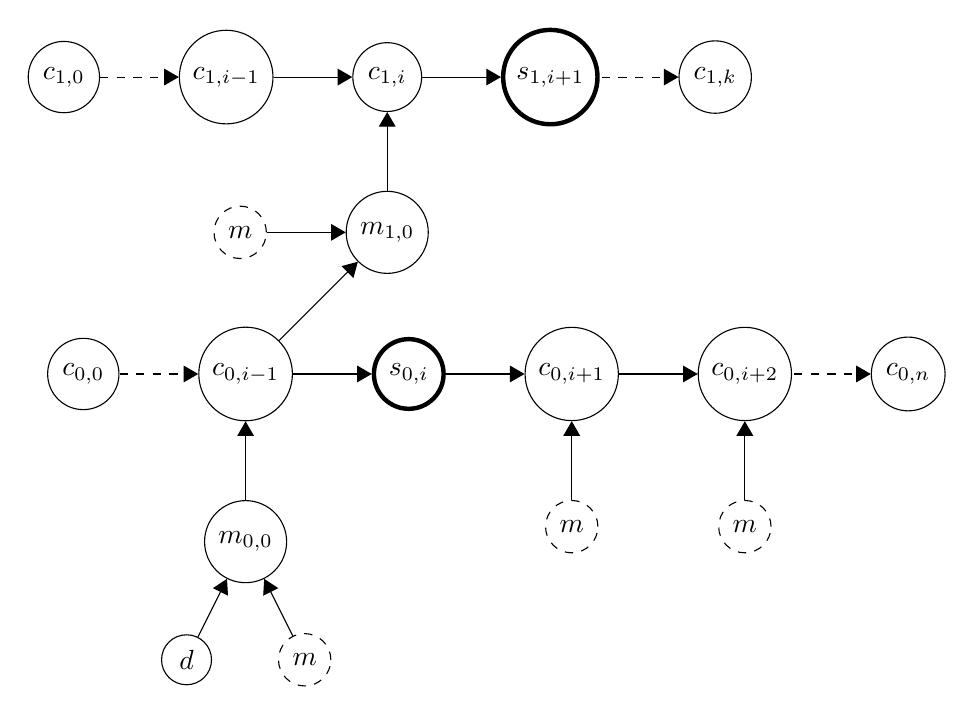
\begin{tikzpicture}[%level/.style={sibling distance=85mm/#1}, 
                                    every node/.style={circle,draw},
                                    every path/.style={<-,>=triangle 60}]

\node[ultra thick] (s0i) {$s_{0,i}$};

\node[left=of s0i] (c0iminus) {$c_{0,i-1}$} edge[->] (s0i);
\node[right=of s0i] (c0iplus) {$c_{0,i+1}$} edge[<-] (s0i);

\node[below=of c0iminus](c0m0) {$m_{0,0}$} edge[->] (c0iminus)
	child {node (d0) {$d$}}
	child {node[dashed] {$m$}};

\node[below=of c0iplus,dashed] {$m$} edge[->] (c0iplus);

\node[left=of c0iminus] (c0) {$c_{0,0}$} edge[->,dashed] (c0iminus);
\node[right=of c0iplus] (c0iplus2) {$c_{0,i+2}$} edge[<-] (c0iplus);

\node[below=of c0iplus2,dashed] {$m$} edge[->] (c0iplus2);

\node[right=of c0iplus2] (c0n) {$c_{0,n}$} edge[<-,dashed] (c0iplus2);


% second dag chain
\node[above right=of c0iminus] (c1m1) {$m_{1,0}$} edge[<-] (c0iminus);
\node[left=of c1m1,dashed] {$m$} edge[->] (c1m1);

\node[above=of c1m1] (c1i) {$c_{1,i}$} edge[<-](c1m1);
\node[left=of c1i] (c1iminus) {$c_{1,i-1}$} edge[->](c1i);
\node[left=of c1iminus] (c10) {$c_{1,0}$} edge[->,dashed](c1iminus);


\node[right=of c1i,ultra thick] (s1iplus) {$s_{1,i+1}$} edge[<-](c1i);

\node[right=of s1iplus] (c1k) {$c_{1,k}$} edge[<-,dashed](s1iplus);


\end{tikzpicture}
        \caption{A directed acyclic graph calendar.}
        \label{fig:dag-overview}
\end{figure}

Figure \ref{fig:dag-overview} shows the basic structure of the DAG calendar. We
show two parallel calendars, $c_0$ and $c_1$, which may be operated by
different entities. From digest $d$ we can trace a path to signature $s_{0,i}$
and another, slightly longer, path to $s_{1,i+1}$. A fully extended timestamp
for that digest including both signatures is now the vertices required to
reproduce the hash chains leading to those two signatures.

The minimum data required to define a vertex in this graph is the tuple
$(d_\mathrm{left},d_\mathrm{right})$, with $d_\mathrm{left}$ and
$d_\mathrm{right}$ defined as the digests of the left and right parent
verticies. The value of a vertex in this scheme is now defined as
$H(d_\mathrm{left}\|d_\mathrm{right})$.

The algorithm to create a timestamp is now the following:

\begin{enumerate}
    \item Generate random nonce $n$
    \item Calculate digest: $d=H(D)+n$
    \item Submit $d$ to server
\end{enumerate}

At this point the digest has been submitted, but the timestamp is not complete.
The server should have responded with some indication of when it will generate
the next calender vertex. Meanwhile the server is doing the following:

\begin{enumerate}
    \item Accept digests from clients
    \item When a calendar time interval has passed, generate optimal balanced
        merkle tree of all submitted digests, and previous calendar digest
    \item Optional: sign calendar head\footnote{The head of the calendar is
        defined as the newest vertex created, whose value no other vertex
        depends on. In some cases there may be multiple heads of the DAG on a
        server.}
    \item Optional: submit calendar head to other servers
    \item Expire old merkle trees, keeping only the calendar itself
\end{enumerate}

To extend the timestamp with all the vertexes in the chain required to validate
a signature(s), the client now does the following:

\begin{enumerate}
    \item Query server with the digest $d$ and a list of identities that the
        client is willing to accept signatures from
    \item Server replies with signature(s) and vertices $v_0$ to $v_n$ required
        to compute a path from $d$ to $s_i$
    \item Save $d$, $n$, $s_0 \dots s_n$, and $v_0 \dots v_n$
\end{enumerate}

The question is, can we make the search operation from $d$ to $s_i$ cheap? We
need the search itself to be fast, and in addition, we need to minimize the
number of steps in any given path so that the space required to store a
timestamp is minimized.

\subsection{Skiplists for optimally short paths}

While we already have an optimally short path from the submitted digest to some
calender vertex, by virtue of combining submitted digests in a single round
using a tree, we do not yet have an optimally short path from calendar vertices
to signatures. Unlike centralized timestamping schemes we can-not guarantee
that a particular calendar vertex will have an acceptable signature; the server
maintaining the calendar may even be totally untrusted. Fortunately there
already exists an append-only data structure with $\log n$ performance:
skiplists.

\begin{figure}
        \centering
        \usetikzlibrary{arrows,positioning}
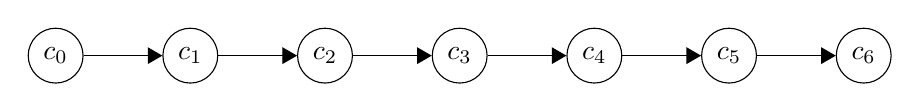
\begin{tikzpicture}[every node/.style={circle,draw},
                                    every path/.style={<-,>=triangle 60}]

\node (c0) {$c_0$};
\node[right=of c0] (c1) {$c_1$} edge (c0);
\node[right=of c1] (c2) {$c_2$} edge (c1);
\node[right=of c2] (c3) {$c_3$} edge (c2);
\node[right=of c3] (c4) {$c_4$} edge (c3);
\node[right=of c4] (c5) {$c_5$} edge (c4);
\node[right=of c5] (c6) {$c_6$} edge (c5);

\end{tikzpicture}
        \caption{A linear calendar.}
        \label{fig:linear-calendar}
\end{figure}

\begin{figure}
        \centering
        \usetikzlibrary{arrows,positioning}
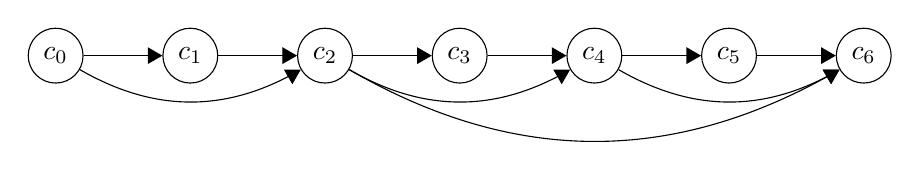
\begin{tikzpicture}[every node/.style={circle,draw},
                                    every path/.style={<-,>=triangle 60}]

\node (c0) {$c_0$};
\node[right=of c0] (c1) {$c_1$} edge (c0);
\node[right=of c1] (c2) {$c_2$} edge (c1) edge[bend left=30] (c0);
\node[right=of c2] (c3) {$c_3$} edge (c2);
\node[right=of c3] (c4) {$c_4$} edge (c3) edge[bend left=30] (c2);
\node[right=of c4] (c5) {$c_5$} edge (c4);
\node[right=of c5] (c6) {$c_6$} edge (c5) edge[bend left=30] (c4) edge[bend left=30] (c2);

\end{tikzpicture}
        \caption{A naive skiplist calendar.}
        \label{fig:naive-skiplist-calendar}
\end{figure}

\begin{figure}
        \centering
        \usetikzlibrary{arrows,positioning}
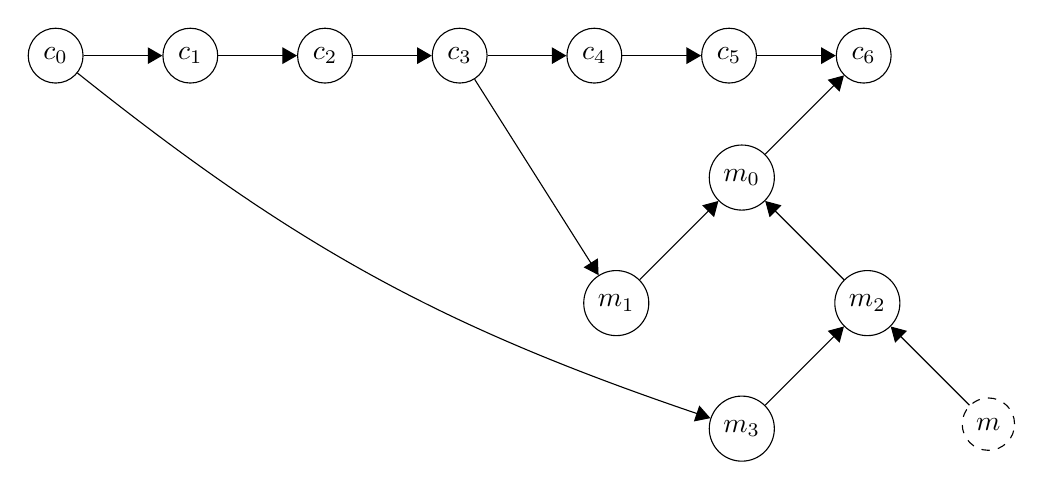
\begin{tikzpicture}[every node/.style={circle,draw},
                                    every path/.style={<-,>=triangle 60}]

\node (c0) {$c_0$};
\node[right=of c0] (c1) {$c_1$} edge (c0);
\node[right=of c1] (c2) {$c_2$} edge (c1);
\node[right=of c2] (c3) {$c_3$} edge (c2);
\node[right=of c3] (c4) {$c_4$} edge (c3);
\node[right=of c4] (c5) {$c_5$} edge (c4);
\node[right=of c5] (c6) {$c_6$} edge (c5);

\node[below left=of c6] (m0) {$m_0$} edge[->] (c6);
\node[below left=of m0] (m1) {$m_1$} edge[->] (m0) edge[<-] (c3);
\node[below right=of m0] (m2) {$m_2$} edge[->] (m0);

\node[below left=of m2] (m3) {$m_3$} edge[->] (m2) edge[bend left=10,<-] (c0);
\node[below right=of m2,dashed] (m4) {$m$} edge[->] (m2);


\end{tikzpicture}
        \caption{A skiplist calendar with all vertices.}
        \label{fig:naive-skiplist-calendar-actual}
\end{figure}

\begin{figure}
        \centering
        \usetikzlibrary{arrows,positioning}
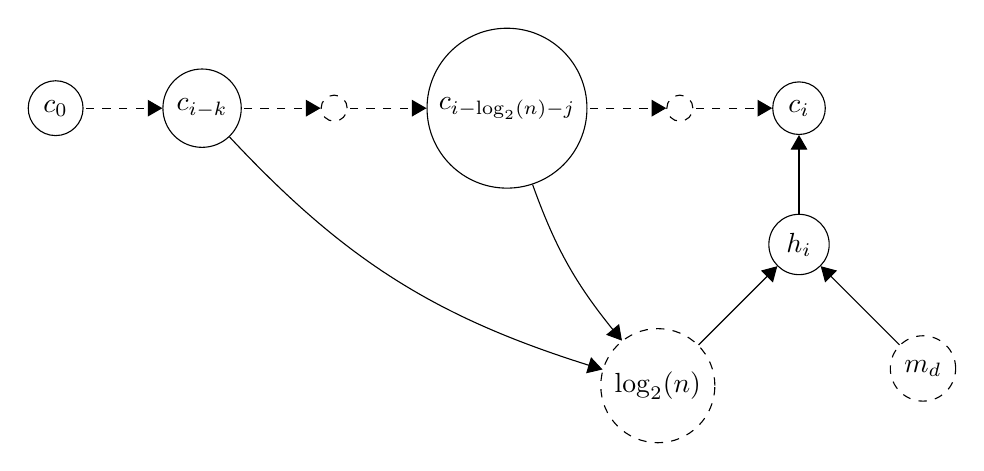
\begin{tikzpicture}[every node/.style={circle,draw},
                                    every path/.style={<-,>=triangle 60}]

\node (c0) {$c_0$};
\node[right=of c0] (ck) {$c_{i-k}$} edge[dashed] (c0);
\node[right=of ck,dashed] (ckmiddle) {} edge[dashed] (ck);
\node[right=of ckmiddle] (ci2){$c_{i-\log_2(n)-j}$} edge[dashed] (ckmiddle);
\node[right=of ci2,dashed] (ci2middle) {} edge[dashed] (ci2);
\node[right=of ci2middle] (ci) {$c_i$} edge[dashed] (ci2middle);

\node[below=of ci] (hi) {$h_i$} edge[->] (ci);
\node[below right=of hi,dashed] (md) {$m_d$} edge[->] (hi);
\node[below left=of hi,dashed] (ms) {$\log_2(n)$} edge[->] (hi) edge[<-,bend left=10] (ci2) edge[<-,bend left=15] (ck);

\end{tikzpicture}
        \caption{A skiplist calendar with all vertices.}
        \label{fig:skiplist-calendar-with-logn-scaling}
\end{figure}

Consider the linear calendar in figure \ref{fig:linear-calendar}. A path from
$c_0$ to $c_6$ will include $5$ additional vertices. Naively, following the
logic of a skiplist, we could add additional edges as shown in figure
\ref{fig:naive-skiplist-calendar}. Now for $n$ calendar vertices in a given
time period, the length of a path between two vertices is bounded by
$\log_2(n)$. The problem the DAG is built by hashing, and every added edge
implies adding a vertex. Figure \ref{fig:naive-skiplist-calendar-actual} shows
a calendar with all extra vertices required; note how the path between $c_3$
and $c_6$ is make no shorter. ($m$ represents the head of the merkle tree for
all submitted digests in the round)

Note that while we could reduce the total \emph{number} of vertices by
concatinating multiple digests together, as opposed to constructing trees, we
would not reduce the \emph{storage} requirements for a paticular timestamp
path.

To determine the optimal depth before inserting a back reference, observe that
an optimal merkle tree linking $n$ digests will leave each digest $\log_2(n)$
steps from the head of the tree. We now say that each calendar vertex with back
references will have the previous calendar vertex as one parent, and a vertex
whose parents in turn are the optimal merkle trees of the back references, and
the digests in that round. Calendar back references are now spaced apart such
that we allow $\log_2(n) + 1 + j$ steps to ``build up'' between the vertex and
the current calendar head, with $j>0$ controlling the balance between timestamp
size and storage requirements for the additional vertexes added. Figure
\ref{fig:skiplist-calendar-with-logn-scaling} shows the resulting graph.

\subsubsection{Skiplist maintenance}

FIXME: Some sort of heap thing? Complex.


\subsection{Finding timestamp paths}

While our data structure results in short paths, we do not yet have a mechanism
for actually finding those paths. To recap we need to find the shortest path
between a given digest $d$ and the oldest signature(s) $S$ signed by a set of
identities $I$. The search algorithm must be efficient even if no path exists;
if the algorithm has poor performance under any circumstance it will allow for
a resource exhaustion attack.

If we could compute the transitive closure\footnote{The transitive closure of a
graph is a graph with all the vertexes of the first, but for every possible
path in the first, an edge is added to the second to allow $O(1)$ reachability
queries.} of the overall hash DAG efficiently our problem would be solved.
Unfortunately the best known dynamic algorithms for this problem have
$O(n^{1.575})$ update performance;\cite{Demetrescu05trade-offsfor} infeasible
for an application which could be adding a minimum of a vertex a second for
years at a time. 

Fortunately in timestamping the DAG has an unusual structure in that any
traversal will soon find itself on the ``main'' calendar path. Suppose we
maintain an invariant known as ``order'', such that for any vertex
$v_\mathrm{order} \ge v_{\mathrm{left}_\mathrm{order}}$ and $v_\mathrm{order}
\ge v_{\mathrm{right}_\mathrm{order}}$

Now lets suppose you wanted to find the path between some vertex, and a
signature vertex. We assume you know the order of the signature vertex - that
data can be easily stored in some sort of sorted list - but not where it is in
the graph. Consider the following recursive python function:

\begin{verbatim}
def walk(starting_vertex,target_vertex,path):
    path = (starting_vertex,path)

    # sorted() by vertex.order
    for next_vertex in \
            sorted(starting_vertex.vertexes_referencing_us,
                   key=lambda x: x.order):

        if next_vertex is target_vertex:
            return (target_vertex,path)
        elif next_vertex.order < target_vertex.order:
            r = walk(next_vertex,target_vertex,(target_vertex,path))
            if r is not None:
                return r
    return None
\end{verbatim}

walk() will either return the path as a linked-list, or None if a path can't be
found. This is fast because it quickly descends deep, as in order, into the
calendar, quickly reaching the target in an optimal number of steps. This is
almost, but not quite, the same traversal function used for a linear skiplist. 

Targetting multiple vertexes at once is a reasonably simple extension:

\begin{verbatim}
def walk(starting_vertex,target_vertexes,path,found_paths):
    path = (starting_vertex,path)

    # sorted() by vertex.order
    for next_vertex in \ 
            sorted(starting_vertex.vertexes_referencing_us,
                   key=lambda x: x.order):

        if next_vertex is in target_vertexes:
            # found one of the targets
            found_paths.append((target_vertex,path))
            target_vertexes.remove(target_vertex)
        elif len(target_vertexes) > 0 \
                and next_vertex.order < max(target_vertexes.order):
            walk(next_vertex,target_vertexes,path,found_paths)
\end{verbatim}

This version is a lot less understandable due to the way it leverages
call-by-reference, in target\_vertexes and found\_paths. There can also be a
minor optimization of pre-calculating max(target\_vertexes.order); that would
be another by-reference function argument. That said, it shows how if searching
for one vertex takes k time, searching for n vertexes will take less than n*k
time.

Note though, we said this algorithm is \emph{almost} the same function as
skiplist traversal. A skiplist traversal function will never backtrack; there
is only one path through the list. If there is a fork in the DAG, such as a
vertex that has been sent to a remote server for timestamping, walk() will
exhaustively search both sides of the fork, as shown in figure
\ref{fig:walk-exhaustive} 





\section{EMAIL}

So I looked up directed acyclic graph search theory.
The comp-sci term for taking a graph, and creating another graph
representing what is connected to what in the first graph, is called
computing the "transitive closure". Unfortunately the problem has been
studied to death and even after decades of research the best performing
algorithms take $O(n^0.58)$ time for a reachibility query, and $O(n^1.58)$
time to add a new vertex to the dag; way too slow. (after all, a slow
query time implies that an attacker can submit a bunch of queries to
bring the server to its knees) This is true whether or not the
transitive closure graph is maintained dynamically, or calculated on
demand.

However, those algorithms are for arbitrary dags. As I said earlier,
mine has the unique property that every element has an obvious ordering,
time. Specifically I'll maintain an invarient, such that for any vertex
v, v.order > v.left.order and v.order > v.right.order This requires
different servers in the network to have clocks set reasonably close to
each other, but it's not disasterous if someone screws that up - their
timestamps will just take longer to get integrated into the dag graphs
of other servers if their clock is set ahead, and if their clock is set
behind, they just take unusually long to integrate other servers
vertexes into their own. The closer in time the clocks are set, the
faster synchronization happens. In extreme cases, say if I set my clock
100 years in the future, you just have to toss out that part of the
graph and start fresh, which isn't a big deal as those timestamps were
invalid anyway. NTP these days works really well.

This ordering should probably be something like a 64-bit unsigned
integer, representing nanoseconds from the UNIX epoch. That gives 500 or
so years until roll over. A subtley is that we'll want to "reserve" some
lower-order bits, so that if we get a bunch of vertexes submitted with
identical orders, we can still construct a valid spanning tree
maintaining the invarient by incrementing linking vertexes by +1.
Alternatively, maybe the inveriant should be >= The order *must* be
part of the data hashed to form the vertex digest. 


The next invarient comes from a related data structure known as a
skiplist. The idea there is to maintain a linked list, with additional
links that "skip" over increasingly larger portions of the list. It
gives the same performence as a binary tree, but with a significantly
simpler implementation. In the graph version you take the set of all
"heads", that is vertexes not referred to by another vertexe's left or
right links, and create a tree of additional vertexes such that for any
randomly picked vertex V there are no more than $\log n$ vertexes between
V and H, the head of the new tree:

      4a
     /
1-2-3
     \
      4b


    /----\
   /  4a  \
  /  /  \  \
1-2-3    5--6
     \  /
      4b

Maintaining this property is required anyway to keep the data required
to store the path data comprising a timestamp small. Currently existing
non-distributed timestamping schemes work by just constructing a optimal
tree from scratch for every round, whose root leaves are the data
submitted for timestamping. But none of those existing schemes support
arbitrary intervals between timestamps, let alone multiple identities
verifying timestamps.


Now lets suppose you wanted to find the path between some vertex, and
signature. (don't forget that a signature itself is stored as a vertex)
You know the order of the signature vertex, (that data can be easily
stored a sorted list) but not where it is in the graph. Consider the
following recursive python function:

\begin{verbatim}
def walk(starting_vertex,target_vertex,path):
    path = (starting_vertex,path)

    # sorted() by vertex.order
    for next_vertex in \
            sorted(starting_vertex.vertexes_referencing_us,
                   key=lambda x: x.order):

        if next_vertex is target_vertex:
            return (target_vertex,path)
        elif next_vertex.order < target_vertex.order:
            r = walk(next_vertex,target_vertex,(target_vertex,path))
            if r is not None:
                return r
    return None
\end{verbatim}

walk() will either return the path as a linked-list, or None if a path
can't be found. This is fast because it quickly descends deep, as in
order, into the tree, quickly reaching the target in an optimal number
of steps. This is almost, but not quite, the same traversal function
used for a linear skiplist. 

Targetting multiple vertexes at once is a reasonably simple extension:

\begin{verbatim}
def walk(starting_vertex,target_vertexes,path,found_paths):
    path = (starting_vertex,path)

    # sorted() by vertex.order
    for next_vertex in \ 
            sorted(starting_vertex.vertexes_referencing_us,
                   key=lambda x: x.order):

        if next_vertex is in target_vertexes:
            # found one of the targets
            found_paths.append((target_vertex,path))
            target_vertexes.remove(target_vertex)
        elif len(target_vertexes) > 0 and next_vertex.order < max(target_vertexes.order):
            walk(next_vertex,target_vertexes,path,found_paths)
\end{verbatim}

This version is a lot less understandable due to the way it leverages
call-by-reference, in target\_vertexes and found\_paths. I also left out
the minor optimization of pre-calculating max(target\_vertexes.order);
that'd be another by-reference function argument. That said, it shows
how if searching for one vertex takes k time, searching for n vertexes
will take less than n*k time.


Note though, I said it's *almost* the same function as skiplist
traversal. A skiplist traversal function will never backtrack; there is
only one path through the list. Consider what happens if there is a fork
in the dag:

\begin{verbatim}
        /-7c-\
     /5a--6a---8a
1-2-3|
     \4b-5b-6b---8b
       \---7b---/
\end{verbatim}

This is a perfectly valid graph by the numerical ordering rule. (drop
the letters) Suppose we start at 1, and are looking for the vertex 8b.
The walk() function will descend 1-2-3-5a-7a-8a, fail, then try 6a, then
finally try 7b-8b. 

Even worse is the result when two graphs get combined, say from taking
over the database of another server:

\begin{verbatim}
1a-2a-3a\
        |-4
1b-2b-3b/
\end{verbatim}

A lookup starting at 1a for a signature at 3b will simply know that it's
looking for a vertex with order three, and exhaustively try every single
vertex in that order range on its side of the graph.


If the master set of identities and signature vertexes was different for
every vertex in the graph this wouldn't be a problem. The query for the
oldest signature at 1a would have returned "there isn't one" and the
lookup could have immediately failed. But how do you efficiently store
that?

An old trick with linked lists, dating back to the lisp days, is that
multiple linked lists can share the same tail, even if the heads are
different. So create a linked-list of signature information. Consider
the vertex DAG: (brackets represent signature vertexes)

\begin{verbatim}
1-2-3-4-(5)-6-7-(8)-9
\end{verbatim}

When vertexes 1 is created, an null linked list is allocated in memory,
and that vertex has a pointer to that linked list. 2-4 then inherit the
same linked list as their parents. (5), the first signature node,
re-writes that shared linked list, so it's tuple value is now (5,null).
The creation of vertex 6 allocates another null list, so the linked list
linked by 1-5 is rewritted again: (5,(null,null)) and 6's pointer now
links to the inner list, (null,null) By the time (8) is created, the
list from vertex 1's perspective is now (5,(8,(null,null)))

However, suppose later in time we need to add a back reference, to
support the dag's log(n) property:

\begin{verbatim}
      /---------------\
1-2-3-4-(5)-6-7-(8)-9-10-(11)
\end{verbatim}

At first glance this looks ok as signature (5) < signature (11), and we
can still lookup newer signatures by just walking the tree.

But what if the two signatures were from different identities? The above
scheme doesn't support multiple identities at all. We can assume that
there will be a lot of identities in the system, keys get compromised
for instance, and anyway we should be able to promiscuously accept
signatures; clients are the ones decided what signatures they'll accept
as trustworthy.

We could store a hash table mapping identities to signature lists, but
then for each vertex you're storing a table with $n$ entries, $n^2$ space
complexity. Caching doesn't work, as an attacker can always bloat the
size of the cache forcing either a time or space attack. There also
isn't any clever way to combine hash tables like there is for lists.

Maybe you could do something with balanced binary trees, but that'd be a
big pile of hidously complex code; people already avoid binary trees
because the standard case is a nightmare to get right. (as an aside, on
the the bitcoin-dev mailing there's some people talking about how to
implement a shared, balanced, deterministic, incrementally updatable in
both addition and deletion, and secure against chosen key attacks
balanced tree as a way to do blockchain compression; if it ever works I
think someone could get a post-doc out of it)

Ultimately putting limits on the size of parallel forks might be the way
to go.


A final problem is how do you actually add those extra vertexes to
maintain the log(n) property? First of all you *must* add the extra
vertexes as the dag grows; as a hash chain vertexes can't be added later
without invalidating the whole tree. 

A standard skiplist has it easy, just link to the $i*n^k$ element in the
list, which can even be directly indexable in memory. Further more you
can easily know how many elements there are in total. The problem here
is that the order gives you no insight into how many edges exist in the
graph between two vertexes. For instance I could add 100 vertexes in a
second, and then wait a few hours to add the next one.

Conceptually, we could maintain the log(n) invarient if whenever a new
vertex was added to the graph, we did a breadth first search starting at
that vertex, and adding an additional linking vertex whenever the depth
walked was greater than log(n)


One possible idea would be to maintain yet another invarient, known as
depth. This property would be a signed integer, with a v.depth >
v.parent.depth invarent, and calculated solely by us.  (unlike order,
where some attacker can manipulate the value; note how if order was
*not* linked to time, an attacker could set it to $2^64-1$...)

Consider the following graph:

\begin{verbatim}
 /----h----\
a-b-c-d-e-f-g
    \-i--/
\end{verbatim}

If a.depth = 0, we can increment depth by 1 for every child vertex.
g.depth will be equal to 6, h.depth = 1, i.depth = 3 

\begin{verbatim}
 /----h----\
a-b-c-d-e-f-g-j-k-l-m
    \-i--/
\end{verbatim}

To recap, for each new vertex added to the
newest part of the graph, extra edges have to be added to older vertexes
in a geometricly decreasing fashion, so that the maximum number of steps
to reach the newest from any older vertex is on the order of log(n). But
how do you do that without walking the graph? If the number of vertexes
per unit time is constant, I'm pretty sure you can just probabilisticly
walk back in time. If it isn't, maybe you need to keep statistics on how
many vertexes in a given order bucket exist, so that your probabilistic
walker works correctly. I don't know the answere to that problem yet.
It's also a problem that has to be handled correctly from the start,
because vertexes can't be changed, and edges can't be added, later in
time.

\bibliographystyle{plain}
\bibliography{paper}

\end{document}
